\chapter{A review on quaternion algebra and its Fourier transform}
\label{ch:reviewQuat}

\begin{quotation}
    \itshape
    And here there dawned on me the notion that we must admit, in some sense, a fourth dimension of space for the purpose of calculating with triples... An electric circuit seemed to close, and a spark flashed forth.

    \noindent --- Sir William Hamilton.
\end{quotation}


In 1833, at the age of 28, Willian Rowan Hamilton presented to the Royal Irish Academy (RIA) a work in which complex numbers were treated as ordered pairs of real numbers, given the appropriate definition of operations\footnote{The results were published in 1837, in the paper \emph{Theory of Conjugate Functions, or Algebraic Couples; with a Preliminary and Elementary Essay on Algebra as the Science of Pure Time} \cite{hamilton1837theory}.}. In the following years, he struggled to extend the complex field into a normed division algebra over triples, but soon realized that, as much as his attempts were inventive, the resulting algebra\footnote{An \textit{algebra over a field}, or simply \textit{algebra}, is a vector space over a field with a bilinear multiplication (that is, the multiplication distributes over the addition and the associativity is valid for multiplication) \cite{schafer1955introduction}.} was not closed under multiplication. We can see this through a simple example \cite{santos2011algebra}: let it be the set $\mathbb{F} = \{ a + b \qi + c \qj  \ | \ (a, b, c) \in \mathbb{R}^3\}$, with $\qi^2 = \qj^2 = -1$ and $\qi \neq \qj$. Since $\qi, \qj \in \mathbb{F}$, so there should exist $x, y, z \in \mathbb{R}$ so that
\begin{equation}
    \qi \qj = x + y \qi + z \qj.
    \label{eq:demonstration01}
\end{equation}

Multiplying by $\qi$ both sides of the equation,
\begin{equation}
    \qi^2 \qj = \qi x + \qi^2 y + z (\qi \qj),
\end{equation}
and using (\ref{eq:demonstration01}) it yields,
\begin{equation}
    - \qj = \qi x - y + z (x + y \qi + z \qj)
    \iff
    (zx - y) + \qi (x + zy) + \qj (z^2 + 1) = 0.
\end{equation}
That is: $z \notin \mathbb{R}$ and $ \qi \qj \notin \mathbb{F} $, proving that such algebraic structure is not closed under multiplication.

Only a decade later, in 1843, while walking by the roads in Dublin towards the RIA, ``an electric circuit seemed to close, and a spark flashed forth'', as he would say. He had conceived the four-dimensional structure required to the desired algebra, creating the quaternions. Moved by excitement, he craved on the stone below Broome Bridge, in Cabra (Dublin), the equations that define the relations between the canonical basis elements of quaternions\footnote{Close to the original site of the inscriptions, the RIA placed a commemorative plaque in 1958, with the same writings.}. This creation, made possible by an insight in 1843, is found accross most of this work. The following sections lead the reader through the foundations of quaternion algebra and quaternion signal analysis.


\section{Introduction to the quaternion algebra}

Quaternions are numbers $q \in \mathbb{H}$ in the form
\begin{equation}
    q = a + b\qi + c\qj + d\qk,
    \label{eq:q}
\end{equation}
in which $a, b, c, d \in \mathbb{R}$, holding true the fundamental relations:
\begin{equation}
    \label{eq:fund_rel}
    \begin{aligned}
        \qi ^2 = \qj^2 & =\qk^2 = \qi \qj \qk = -1.
    \end{aligned}
\end{equation}

The multiplication rules between  $ \qi $, $ \qj $ and $ \qk $ follow directly from (\ref{eq:fund_rel}), resembling those between orthonormal basis vectors from $ \mathbb{R}^3 $ and the vector product: the product between two of them yields the third, the sign being determined from the operands order. For instance, to find the result of $ \qi \qj $ one may start from (\ref{eq:fund_rel}) and write
\begin{equation}
    \begin{aligned}
        \qi \qj \qk                         & = -1   \\
        \qi \qj \underbrace{\qk \qk}_{= -1} & = -\qk \\
        \qi \qj                             & = \qk.
    \end{aligned}
\end{equation}
Similarly, to find $ \qj \qi $,
\begin{equation}
    \begin{aligned}
        \qi \qj \qk     & = -1        \\
        \qi \qi \qj \qk & = -\qi      \\
        - \qj \qk       & = - \qi     \\
        \qj \qj \qk     & =  \qj \qi  \\
        - \qk           & =  \qj \qi. \\
    \end{aligned}
\end{equation}
Fig. \ref{fig:quatmult} depicts the order in which the product between any pair in the triplet $ \qi $, $ \qj $ and $ \qk $ yields the third one, with positive sign. All three units commute with real numbers. The most relevant consequence, therefore, of (\ref{eq:fund_rel}), is that the quaternion product is \textit{noncommutative}. In fact, it is the first example of noncommutative normed division algebra in history \cite{kleiner2007history}.

\begin{figure}
    \centering
    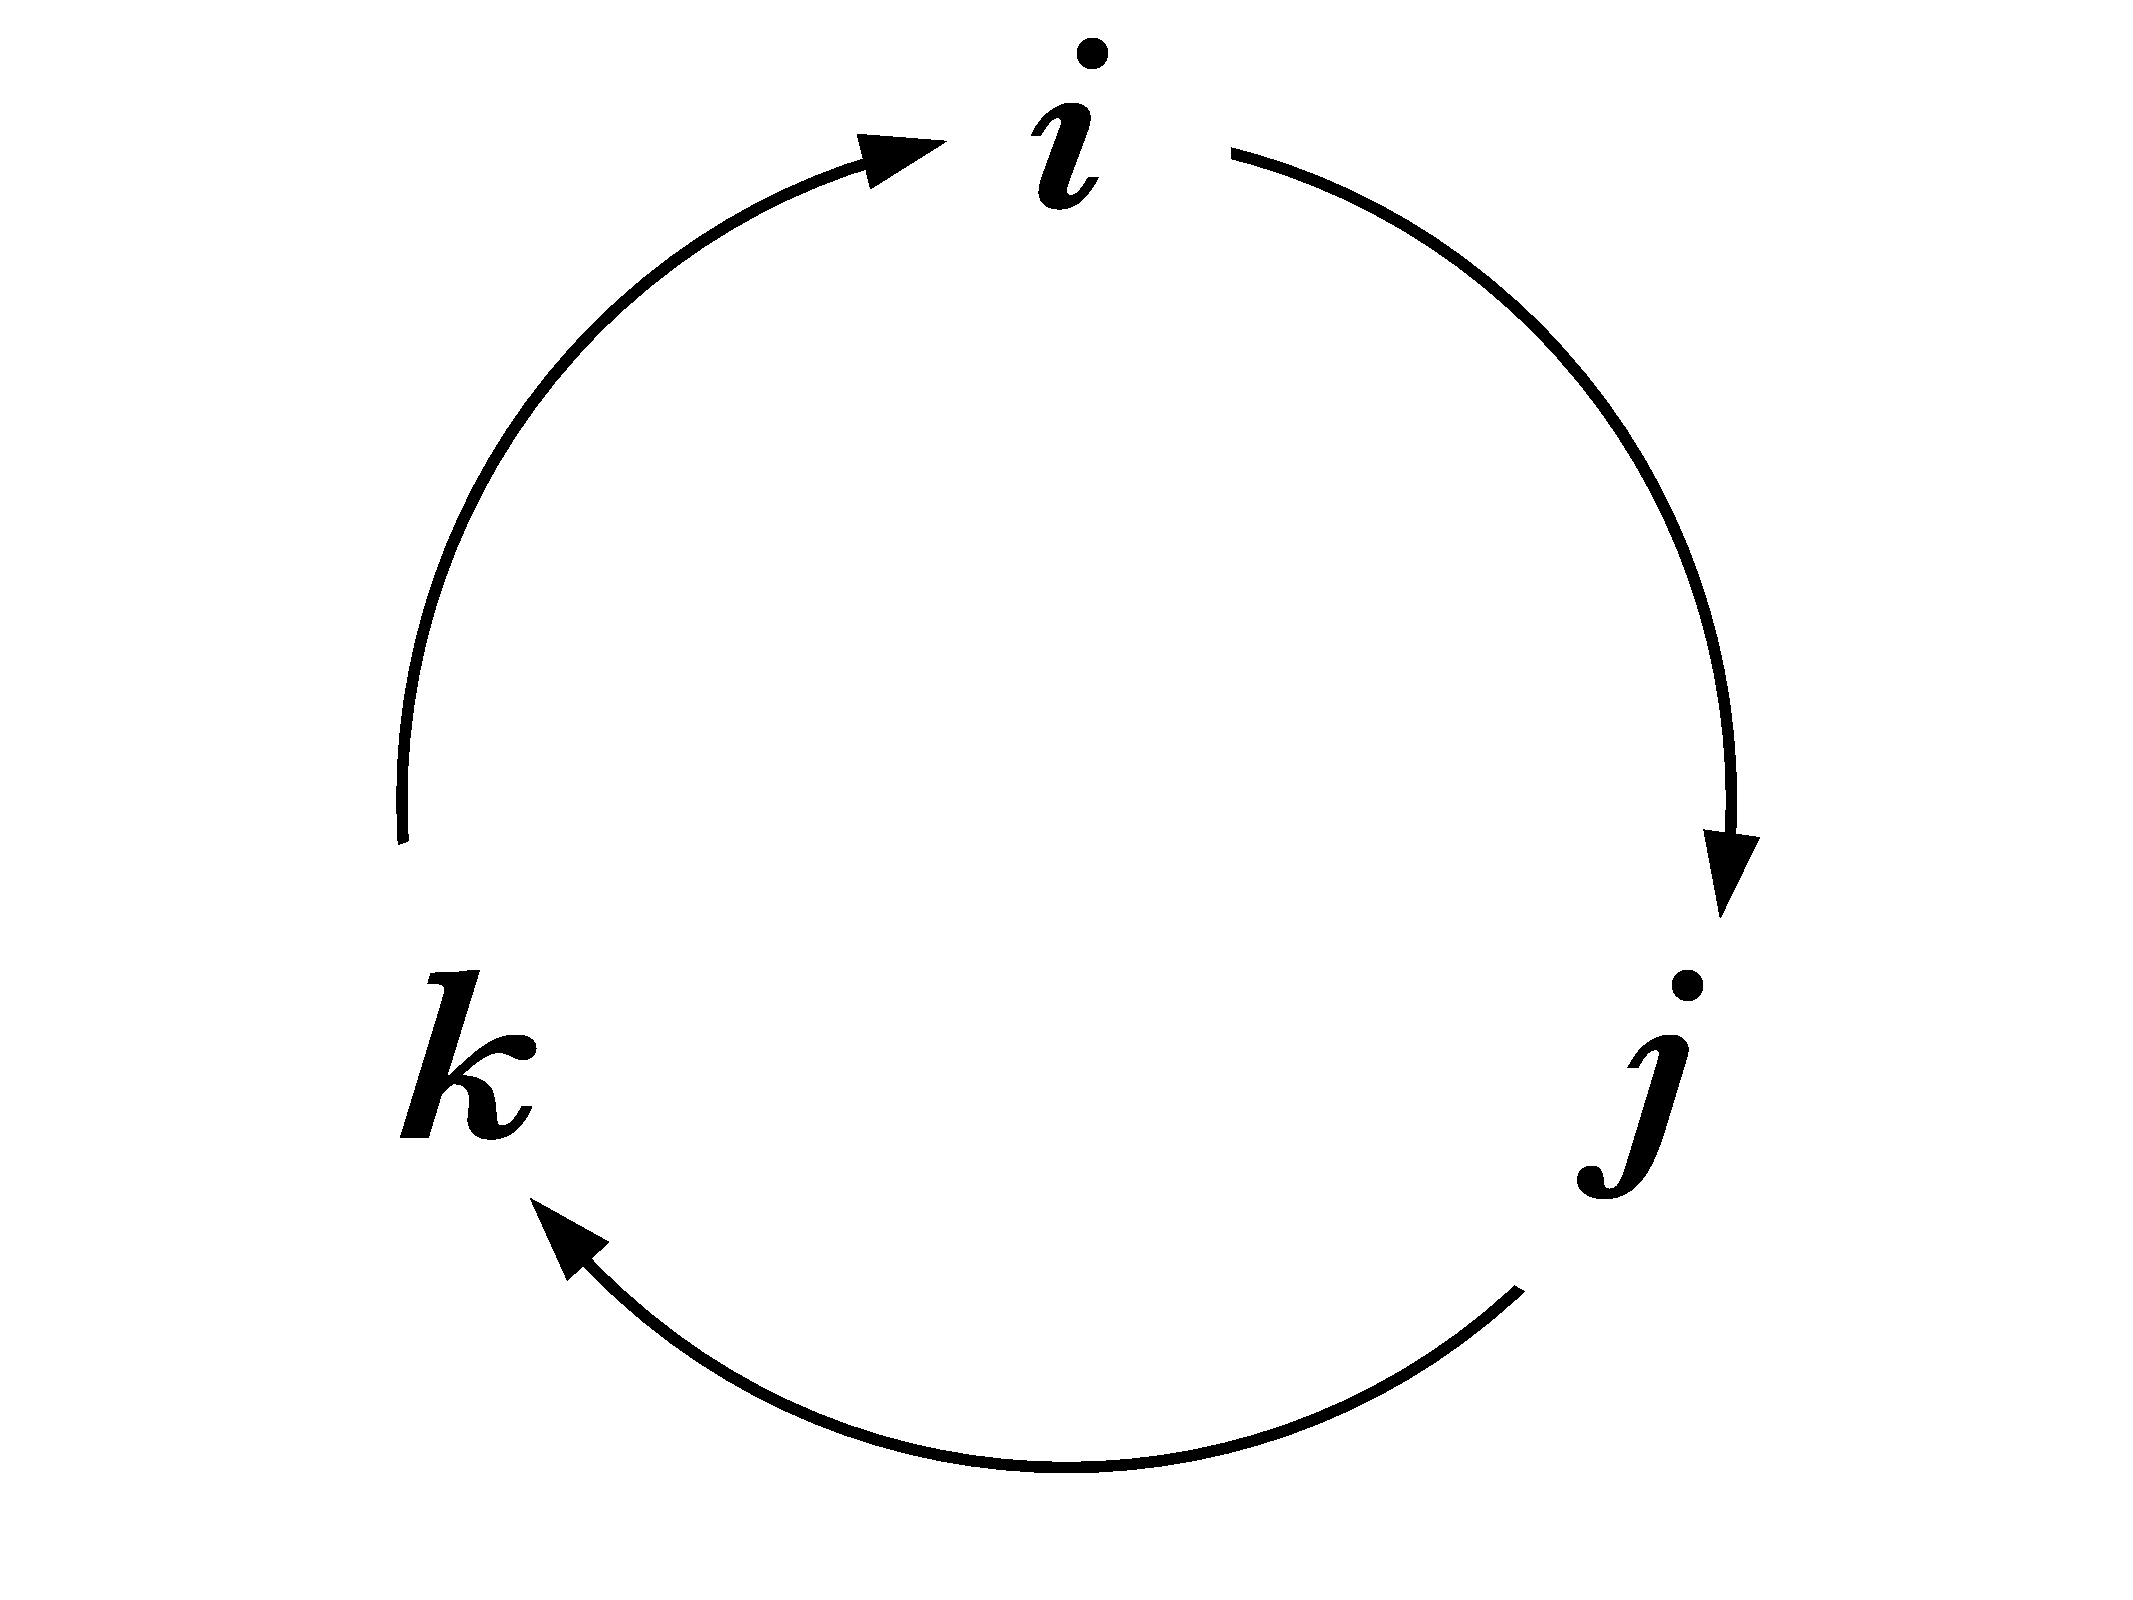
\includegraphics[width=0.2\linewidth]{Figures/quaternion_multiplication.pdf}
    \caption{Illustration of the multiplication rule between the imaginary units $ \qi $, $ \qj $ and $ \qk $.}
    \label{fig:quatmult}
\end{figure}

The exploration of the quaternion multiplication rules gives rise to a useful property, related to products between complex numbers and elements from the quaternion canonical basis. In particular, the product between $\qj$ and any complex number $x = a + b \qi , \ a, b \in \mathbb{R}$, satisfies $\qj x = \overline{x} \qj$, since
\begin{equation}
    \label{eq:commutej}
    \begin{aligned}
        \qj x & = \qj (x_r + x_i \qi) = x_r \qj + x_i \qj \qi = x_r \qj - x_i \qi \qj \\
              & = (x_r - x_i \qi) \qj = \overline{x} \qj.
    \end{aligned}
\end{equation}
This will come up a couple of times during manipulations in this thesis.

The elements $\qi, \qj$ e $\qk$ may be perceived as orthogonal imaginary units, generating the 3D space of quaternion \textit{imaginary parts},
\begin{equation}
    \qV (q) = b\qi + c\qj + d\qk.
\end{equation}
The \emph{real part} of a quaternion \emph{q} is defined as
\begin{equation}
    S(q) = a.
\end{equation}

The imaginary part is usually referred to as \textit{vector part}, while the real part may also be called \textit{scalar part}. A quaternion with null real part is said to be \textit{pure} --- the set of which is represented by $\qV(\mathbb{H})$. The product between pure quaternions may be written similarly to that between $\mathbb{R}^3$ vectors, i.~e., if $v_1 = b_1\qi + c_1\qj + d_1\qk$ and $v_2 = b_2\qi + c_2\qj + d_2\qk$, then
\begin{equation}
    v_1 \times v_2 =
    \begin{vmatrix}
        \qi & \qj & \qk \\
        b_1 & c_1 & d_1 \\
        b_2 & c_2 & d_2
    \end{vmatrix}.
\end{equation}

Based on the similarity between the $ \mathbb{R}^3 $ set, equipped with the cross product, and the set of pure quaternions, equipped with their quaternion product, it is usual to refer to $\qi, \qj$ and $\qk$ as \emph{axis}. The term references the interpretation of theses imaginary units as being coordinate axis in the 3D space of pure quaternions.

The analogy with the $\mathbb{R}^3$ vector operations also extends to the definition of inner product between pure quaternions $v_1 = b_1\qi + c_1\qj + d_1\qk$ and $v_2 = b_2\qi + c_2\qj + d_2\qk$:
\begin{equation}
    \langle v_1, v_2 \rangle =
    b_1 b_2 + c_1 c_2 + d_1 d_2.
\end{equation}

The quaternion multiplication distributes over quaternion addition
% this english sentence is right: https://en.wikipedia.org/wiki/Distributive_property
and is also associative. That is, if $q_1 = a_1 + b_1\qi + c_1\qj + d_1\qk$ and $q_2 = a_2 +  b_2\qi + c_2\qj + d_2\qk$, then their sum is simply
\begin{equation}
    q_1 + q_2 = (a_1 + a_2) + (b_1 + b_2)\qi + (c_1 + c_2)\qj + (d_1 + d_2)\qk,
\end{equation}
whereas their product is
\begin{equation}
    \label{eq:q_prod}
    \begin{aligned}
        q_1 q_2 = & \ (a_1 + b_1\qi + c_1\qj + d_1\qk) (a_2 +  b_2\qi + c_2\qj + d_2\qk) \\
        =         & \ (a_1 a_2 - b_1 b_2 - c_1 c_2 - d_1 d_2)                            \\
                  & + \qi (b_1 a_2 + a_1 b_2 - d_1 c_2 + c_1 d_2)                        \\
                  & + \qj (c_1 a_2 + d_1 b_2 + a_1 c_2 - b_1 d_2)                        \\
                  & + \qk (d_1 a_2 - c_1 b_2 + b_1 c_2 + a_1 d_2).
    \end{aligned}
\end{equation}

Finally, it is possible to write the quaternion product in (\ref{eq:q_prod}) as a function of the operands scalar and vector parts,
\begin{equation}
    \label{eq:prod_vectors}
    \begin{aligned}
        q_1 q_2 = & \ S(q_1)S(q_2) - \langle\qV(q_1), \qV(q_2)\rangle              \\
                  & + S(q_1) \qV(q_2) + S(q_2)\qV(q_1) + \qV(q_1) \times \qV(q_2).
    \end{aligned}
\end{equation}
The lack of commutativity in the cross product is another demonstration of the fact that quaternion multiplication is noncommutative.

Quaternion conjugation, as defined in the complex numbers, is obtained changing the sign of the imaginary part: $ \bar{q} \overset{\Delta}{=} S(q) - \qV(q) $. The quaternion \textit{norm} is defined as $\Vert q \Vert \overset{\Delta}{=} a^2 + b^2 + c^2 + d^2 = q \bar{q} = \bar{q} q$, whereas the \textit{modulus} of $q$ \cite{ell2014quaternion} is
\begin{equation}
    \label{eq:modulusq}
    |q| \overset{\Delta}{=} \sqrt{a^2 + b^2 + c^2 + d^2} = \Vert q \Vert^{\nicefrac{1}{2}}.
\end{equation}

From the definition of quaternion conjugation, the product between the conjugate of two quaternions $q$ and $p$ equals
\begin{equation}
    \begin{aligned}
        \bar{q} \bar{p} & =
        \left[ S(q) - \qV(q) \right] \left[ S(p) - \qV(p) \right]               \\
                        & = S(q)S(p) - \qV(q) S(p) - S(q) \qV(p) + \qV(q)\qV(p) \\
                        & = S(q)S(p) - S(p)\qV(q) - S(q) \qV(p) + \qV(q)\qV(p).
    \end{aligned}
\end{equation}
From (\ref{eq:prod_vectors}),
\begin{equation}
    \qV(q) \qV(p) =
    \qV(q) \times \qV(p) - \langle\qV(q), \qV(p)\rangle =
    - \qV(p) \qV(q),
\end{equation}
therefore
\begin{equation}
    \bar{q} \bar{p} =
    S(q)S(p) - S(p)\qV(q) - S(q) \qV(p) - \qV(p)\qV(q) =
    \overline{p q},
\end{equation}
showing that $\bar{q} \bar{p} = \overline{p q}$. This result allows to prove that $\Vert p q \Vert = \Vert p \Vert \Vert q \Vert$, since
\begin{equation}
    \label{eq:normproduct}
    \begin{aligned}
        \Vert pq \Vert = \overline{pq} pq = \bar{q} \bar{p} p q = \bar{q} \Vert p \Vert q = \Vert p \Vert \bar{q} q =
        \Vert p \Vert \Vert q \Vert.
    \end{aligned}
\end{equation}

A \textit{unit} quaternion has, by definition, unit norm, and the norm definition also leads to the quaternion multiplicative inverse (if $q \neq 0$),
\begin{equation}
    q^{-1} = \frac{\bar{q}}{\Vert q \Vert}.
\end{equation}

From the analogy between pure quaternions and the elements in $ \mathbb{R}^3 $, the idea of perpendicularity between pure quaternions presents itself naturally. Given $ \qmu,  \qnu \in \qV(\mathbb{H})$, they are said orthogonal --- we write $ \qmu \perp \qnu $ --- if and only if
\begin{equation}
    S(\qmu \qnu) = \langle \qmu, \qnu \rangle = 0.
    % \tag{$ \iff \qmu \perp \qnu $}
\end{equation}
For two orthogonal unit pure quaternions $ \qmu $ and $ \qnu $, it follows from (\ref{eq:prod_vectors}) that $ \qmu \qnu  = \qmu \times \qnu$, therefore $ \qmu \qnu \perp \qmu $ and $ \qmu \qnu \perp \qnu $. Since $ (\qmu, \qnu, \qmu \qnu) $ is a triplet of orthogonal unit pure quaternions, they form a basis for $ \qV (\mathbb{H}) $. Hence it is possible to rewrite (\ref{eq:q}) as
\begin{equation}
    \label{eq:quat_generalizado}
    q = a + b'\qmu + c'\qnu + d'\qmu \qnu,
\end{equation}
$a, b', c', d' \in \mathbb{R}$,
which represents the so called \emph{generalized quaternion}. The \emph{classical Hamiltonian quaternions} are those written in terms of the canonical basis $ (1, \qi, \qj, \qk) $.


Besides the cartesian representation (\ref{eq:q}), quaternions allow the so called \emph{Euler form} \cite{ell2014quaternion}, a polar representation commonly expressed as
\begin{equation}
    \label{eq:euler}
    q = |q| e^{\qmu \theta} = |q|\cos \theta + |q|\qmu \sen \theta,
\end{equation}
in which $ \qmu $ is a unit pure quaternion, parallel to the vector part of $ q $.

As a remarkable consequence of (\ref{eq:euler}), it follows that every unit pure quaternion is a square root of $-1$. For instance, let $ \qnu $ be a unit pure quaternion. From (\ref{eq:euler}),
\begin{equation}
    %\label{key}
    \qnu = |\qnu| e^{\qnu \theta},
\end{equation}
but since $ |\qnu| = 1 $, then
\begin{equation}
    %\label{key}
    \qnu = e^{\qnu \theta}  = \cos \theta + \qnu \sen \theta \Rightarrow \theta = \frac{\pi}{2},
\end{equation}
hence,
\begin{equation}
    %\label{key}
    \qnu^2 = \left( e^{ \qnu \frac{\pi}{2}} \right)^2 = e^{\qnu \pi} = \cos \pi + \qnu \sen \pi = -1.
\end{equation}

This property leads to the conclusion that numbers such as $ a + \qmu b  $ form an isomorphism with the complex numbers. For this reason, the set composed by such numbers is represented by $ \mathbb{C}_{\qmu} \overset{\Delta}{=} \{ a + \qmu b \ |\  a, b \in \mathbb{R} \}$ (and hence $ \mathbb{C}_{\qi} $ can be identified, for all practical ends, as the usual set of complex numbers, by making the extrapolation that the unit pure quaternion $\qi$ equals the complex imaginary unit).

Another crucial representation of quaternion numbers is called \emph{symplectic decomposition}. Every quaternion $ q = a + b\qi + c\qj + d\qk \in \mathbb{H} $ can be represented as
\begin{equation}
    q = q_1 + q_2 \qj, \quad q_1, q_2 \in \mathbb{C}_{\qi},
\end{equation}
in which the complex numbers $ q_1 = a + b\qi $ and $ q_2 = c + d\qi $ are commonly named \emph{simplex} and \emph{perplex} parts, respectively. In general, the decomposition does not need to take $\qi$ as reference axis. Take for example $ \qmu $ and $ \qnu $ as arbitrary orthogonal unit pure quaternions, hence any quaternion $ q $ may be decomposed as
\begin{equation}
    \label{eq:decomposicao}
    q = q_1 + q_2 \qnu, \quad q_1, q_2 \in \mathbb{C}_{\qmu}.
\end{equation}
That is a hugely important tool when it comes to computing the QDFT (see Section \ref{sec:QFT}) and handling quaternion matrices (cf. Chapter \ref{ch:QGSP}).

\subsection{Quaternion similarity and rotation}
\label{subsec:rotacionando}
Two quaternions $ q $ and $ r $ are said to be \emph{similar} if it exists a non-zero quaternion $ v $ such that $ v^{-1}q v = r $. In this case, one can write $ q \sim r $. Similarity between quaternions constitutes an equivalence relation \cite{zhang1997quaternions}, and all elements from a same similarity class possess the same norm, since, from (\ref{eq:normproduct}), $ |v^{-1}q v| = |v^{-1}| \cdot |q| \cdot |v| = |q| $.

It matters to notice that an important property of quaternion similarity transformations, which justifies its great use in mechanics and graphics computing industry, is that it performs a rotation on the $\qi \qj \qk$ space. Given $ v,q \in \mathbb{H} $, $ v = |v| e^{\qmu \alpha}$, the similarity transformation
\begin{equation}
    \label{eq:rotacao}
    \phi_v(q) = v q v^{-1}
\end{equation}
produces the rotation of the vector part of $q$ along the axis $ \qmu $ (which is parallel to the vector part of $v$) through an angle $ 2\alpha $ \cite{ward2012quaternions}, following the right-hand rule. Let us illustrate this property with an example.

\vspace{-2em}
\begin{quotation}
    \begin{example}
        \label{example:01}
        \upshape
        Let $ \lambda = 3\qi + \qk $ and
        \begin{equation}
            %\label{key}
            \mathbf{v} =\begin{pmatrix}
                1 +  \qi \\
                2 \qj + \qk
            \end{pmatrix}
        \end{equation}
        be, respectively, an eigenvalue and its eigenvector of a matrix $\mathbf{A} \in \mathbb{H}^{2 \times 2}$. The eigenvalue problem over the quaternions will be introduced in the next section, so let us not consider its details for now. It suffices to know that $\lambda$, $\mathbf{A}$ and $\mathbf{v}$ satisfy the equation
        \begin{equation}
            \label{eq:03}
            \mathbf{A} \mathbf{v} = \mathbf{v} \lambda.
        \end{equation}

        Let us restrict the first column of $\mathbf{A}$ to be equal to $ (1 \quad 1)^T $, so that the the matrix is now fully determined,
        \begin{equation}
            %\label{key}
            \mathbf{A} =
            \begin{pmatrix}
                1 & - \frac{1}{5} + \frac{3}{5} \qi + 2 \qj \\
                1 & -3 \qi + \qj
            \end{pmatrix}.
        \end{equation}

        Given an invertible quaternion $q$, the equation may be rewritten as
        \begin{equation}
            \label{eq:rewritten}
            \mathbf{A} (\mathbf{v} q) = (\mathbf{v} q) q^{-1} \lambda q,
        \end{equation}
        which presents the similarity transformation $q^{-1} \lambda q$. Since similar quaternions differ only by a rotation of their vector parts, it is clearly possible to find a quaternion $q$ so that the vector part of $q^{-1} \lambda q$ is parallel to $\qi$ --- that is, $q^{-1} \lambda q$ is a complex number. Let us go through that process.

        Since the vector part of $\lambda$ belongs to the $ \qi \qk $ plane, the idea is to use (\ref{eq:rotacao}) to rotate $\lambda$ along the $\qj$ axis (orthogonal to the rotation plane) by an angle of $ \theta = \tan^{-1} \frac{1}{3} $ radians, towards $ \qi $ (see Fig. \ref{fig:quat3ik}). The required quaternion to enable such rotation is, therefore,
        \begin{equation}
            \label{eq:04}
            v = e^{\qj \alpha}, \quad 2\alpha = \theta = \tan^{-1} \frac{1}{3},
        \end{equation}
        using the mapping $ \lambda \mapsto v \lambda v^{-1} $ in (\ref{eq:rotacao}).

        \begin{figure}
            \centering
            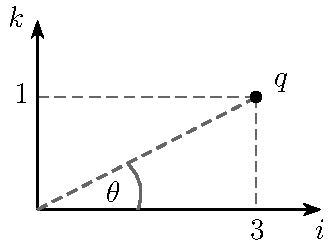
\includegraphics[width=0.25\linewidth]{Figures/quaternion01.pdf}
            \caption{Representation of $ \lambda = 3\qi + \qk $ in the $ \qi \qk $ plane.}
            \label{fig:quat3ik}
        \end{figure}

        Recalling that our desired transformation is written as $ \lambda \mapsto q^{-1} \lambda q $, then
        \begin{equation}
            %\label{key}
            q = v^{-1} = e^{- \qj \alpha} = e^{- \qj \frac{\theta}{2}}.
        \end{equation}

        As a sanity check, let us find the value of $ \alpha $ which results in $ q^{-1} \lambda q \in \mathbb{C}_{\qi} $. Since $ v = q^{-1} = \cos \alpha + \qj \sin \alpha $,
        \begin{equation}
            %\label{key}
            \begin{aligned}
                %\label{key}
                q^{-1} \lambda   & = (\cos \alpha + \qj \sin \alpha)(3 \qi + \qk)                                                          \\
                                 & = \qi(3 \cos \alpha + \sin \alpha) + \qk(\cos \alpha - 3 \sin \alpha).                                  \\
                q^{-1} \lambda q & = [\qi(3 \cos \alpha + \sin \alpha) + \qk(\cos \alpha - 3 \sin \alpha)] (\cos \alpha - \qj \sin \alpha) \\
                                 & = \qi (3 \cos 2\alpha + \sin 2\alpha) + \qk(\cos 2\alpha - 3 \sin 2\alpha).
            \end{aligned}
        \end{equation}

        Therefore, $ q^{-1} \lambda q \in \mathbb{C}_{\qi} $ if and only if
        \begin{equation}
            %\label{key}
            \begin{aligned}\textbf{}
                \cos 2\alpha - 3 \sin 2\alpha & = 0                      \\
                \Rightarrow 2\alpha           & = \tan^{-1} \frac{1}{3},
            \end{aligned}
        \end{equation}
        as determined by (\ref{eq:04}).

        Consequently, it was demonstrated that the unit pure quaternion $ q = e^{- \qj \alpha} $, with $ \alpha = - \displaystyle \nicefrac{1}{2} \tan^{-1} \nicefrac{1}{3} $, produces, through a similarity transformation, the complex-valued eigenvalue $ q^{-1} \lambda q \in \mathbb{C}_{\qi}$. Since $q = \cos \alpha - \qj \sin \alpha $, (\ref{eq:03}) can be rewritten as in (\ref{eq:rewritten}),
        \begin{equation}
            %\label{key}
            \mathbf{A} \underbrace{\begin{pmatrix}
                    cos \alpha + \qi \sin \alpha - \qj \sin \alpha - \qk \sin \alpha \\
                    2 \sin \alpha + \qi \sin \alpha + \qj 2 \cos \alpha + \qk \cos \alpha
                \end{pmatrix}}_{= \mathbf{v} q} =
            (\mathbf{v} q) \cdot \underbrace{\qi (3 \cos 2\alpha + \sin 2\alpha)}_{= q^{-1} \lambda q}.
            %\underbrace{3.162 \qi}_{= \bar{u} q u}.
        \end{equation}
        Let us leave a remark for the user, as an anticipation of the upcoming section: notice how $\mathbf{v}$ and $\mathbf{v}q$ are the same eigenvector up to a scaling factor, and it is always possible to make $q^{-1} \lambda q$ into a complex number through a similarity transformation, given that the vector part of $\lambda$ has non-zero norm.
    \end{example}
\end{quotation}


\section{On the theory of quaternion matrices}

When analyzing the eigenstructure and subsequent fractionalization of the QDFT matrix, the eigendecomposition of the DFT and the eigenvector sharing served as a convenient shortcut. In order to build the results in QGSP, however, it is required to dive into more general properties of quaternion matrices. The symplectic decomposition, already presented in (\ref{eq:decomposicao}), plays an important role in that matter, specialy for its use in defining the \textit{complex adjoint matrix}.

\begin{definition}[Complex adjoint matrix \cite{zhang1997quaternions}]
    \label{def:complexadjoint}
    Given $ \mathbf{A} \in \mathbb{H}^{n \times n} $, with symplectic decomposition $ \mathbf{A}_1 + \mathbf{A}_2 \qj$, $ \mathbf{A}_1,\mathbf{A}_2 \in \mathbb{C}^{n \times n} $, its complex adjoint matrix is defined as
    \begin{equation}
        \rchi_{A} \overset{\Delta}{=}
        \begin{pmatrix}
            \mathbf{A}_1              & \mathbf{A}_2            \\
            - \overline{\mathbf{A}}_2 & \overline{\mathbf{A}}_1
        \end{pmatrix}.
    \end{equation}
\end{definition}

In the following theorems, Zhang brings fundamental results for building QGSP.

\begin{theorem}[Part of Theorem 4.2 in
        \cite{zhang1997quaternions}
    ]
    \label{th:equiv01}
    Given the matrix $ \mathbf{A} \in \mathbb{H}^{n \times n} $, the following sentences are equivalent:

    \begin{itemize}[noitemsep]
        \item $ \rchi_{AB} = \rchi_{A} \rchi_{B} $,
        \item $ \rchi_{A^{-1}} = \rchi_{A}^{-1}$, if $ \mathbf{A}^{-1} $ exists,
        \item $ \rchi_{A}$ is unitary, Hermitian or normal if and only if so is $ \mathbf{A} $.
    \end{itemize}

\end{theorem}

\begin{theorem}[Part of Theorem 4.3 in
        \cite{zhang1997quaternions}
    ]
    \label{th:equiv02}
    Given the matrix $ \mathbf{A} \in \mathbb{H}^{n \times n} $, the following sentences are equivalent:

    \begin{itemize}[noitemsep]
        \item $\mathbf{A}$ is invertible.
        \item $\mathrm{det}(\rchi_A) \neq 0$, i.~e., $\rchi_{A}$ is invertible.
    \end{itemize}

\end{theorem}

Differently from other representations of quaternion matrices in $ \mathbb{C} $ or $ \mathbb{R} $, the complex adjoint allows to establish an important relation between the spectra of $ \rchi_{A} $ and $ \mathbf{A} $, as will soon be discussed.

\subsection{Eigenvalues}
Since quaternion multiplication is noncommutative, it is necessary to distinguish between \textit{left} and \textit{right} eigenvalues of a given matrix $ \mathbf{A} \in \mathbb{H}^{n \times n} $,
\begin{align*}
    \mathbf{A} \mathbf{v} & = \mathbf{v} \lambda, \tag{right} \\
    \mathbf{A} \mathbf{v} & = \lambda \mathbf{v}.  \tag{left}
\end{align*}

We will restrict this discussion mostly to right eigenvalues, since they hold a broader set of results in literature \cite[Cap. 5]{zhang1997quaternions} and are, for that matter, a safer point of support when developing QGSP. When not explicitly mentioned, the right eigenvalues will simply be referred to as \textit{eigenvalues} of the quaternion matrix.

It matters to highlight the fact that a quaternion matrix possesses a \textit{finite} number of eigenvalues if and only if they are all real-valued. Otherwise, each of them will belong to a similarity class, according to the transformation $ \lambda_1 = q^{-1} \lambda_2 q $, containing \textit{infinite} quaternions which are also eigenvalues of the same matrix (return to Example \ref{example:01}, for instance). Let $ \lambda $ be an eigenvalue of the matrix $ \mathbf{A} $ associated with the eigenvector $ \mathbf{v} $. That is,
\begin{equation}
    \begin{aligned}
        \label{eq:similar}
        \mathbf{A} \mathbf{v}     & = \mathbf{v} \lambda                                   \\
        \mathbf{A} \mathbf{v} q   & = \mathbf{v} \lambda q = \mathbf{v} q q^{-1} \lambda q \\
        \mathbf{A} (\mathbf{v} q) & = (\mathbf{v} q) q^{-1} \lambda q,
    \end{aligned}
\end{equation}
so that $ q^{-1} \lambda q $ is an eigenvalue associated with the eigenvector $ \mathbf{v}q $, with $ q \in \mathbb{H}^\ast $.

\subsection{Diagonalizability}
\label{subsec:autovetores_XA}

The problem of quaternion matrix diagonalization differs greatly from the case with complex matrices. In the latter scenario, having no pair of equal eigenvalues is a sufficient condition for diaginalizability, but the rule does not hold for the quaternio case. See for instance the counterexample given by Zhang \cite[Exemplo 7.4]{zhang1997quaternions}, the matrix
\begin{equation}
    \mathbf{A} =
    \begin{pmatrix}
        \qi & 1   \\
        0   & \qj
    \end{pmatrix}.
\end{equation}

Although its eigenvalues are distinct -- $ \qi $ and $ \qj $, since they lie on the main diagonal of an upper triangular matrix --, the respective eigenvectors do not constitute a linearly independent set. Notice, for example, that an eigenvector associated with $ \qi $ is $ (1, 0)^T $, whereas one associated with $ \qj $ is $ (\qi + \qj, 0)^T $. The reason as to why they form a linearly dependent set is the fact previously stated that, for each eigenvalue and eigenvector $ \lambda $ and $ \mathbf{v} $ from a quaternion matrix, it follows that $ q^{-1}\lambda q $ and $ \mathbf{v}q $ form another eigenvalue-eigenvector pair, with $ q \in \mathbb{H}^\ast $. That is, two \emph{similar} eigenvalues are always associated with the same eigenvector (up to a scaling factor). That is why similar quaternions are said to belong to the same \emph{eigenclass} \cite{de2000right}. In order to have a linearly independent set of eigenvectors, therefore, their eigenvalues must not be similar. Concluding the counterexample, the reader may show that $ \qi $ and $ \qj $ satisfy the similarity relation $ \qj = q \qi q^{-1} $ whenever $q$ belongs to the set $ \{ a - a\qi - a\qj + a\qk \ | \ a\in \mathbb{R}^\ast \} $.

Theorem \ref{th:02} relates the eigendecomposition of a quaternion matrix to that of its complex adjoint, providing a fundamental principle to the study of quaternions matrices eigenstructure.

\begin{figure}
    \centering
    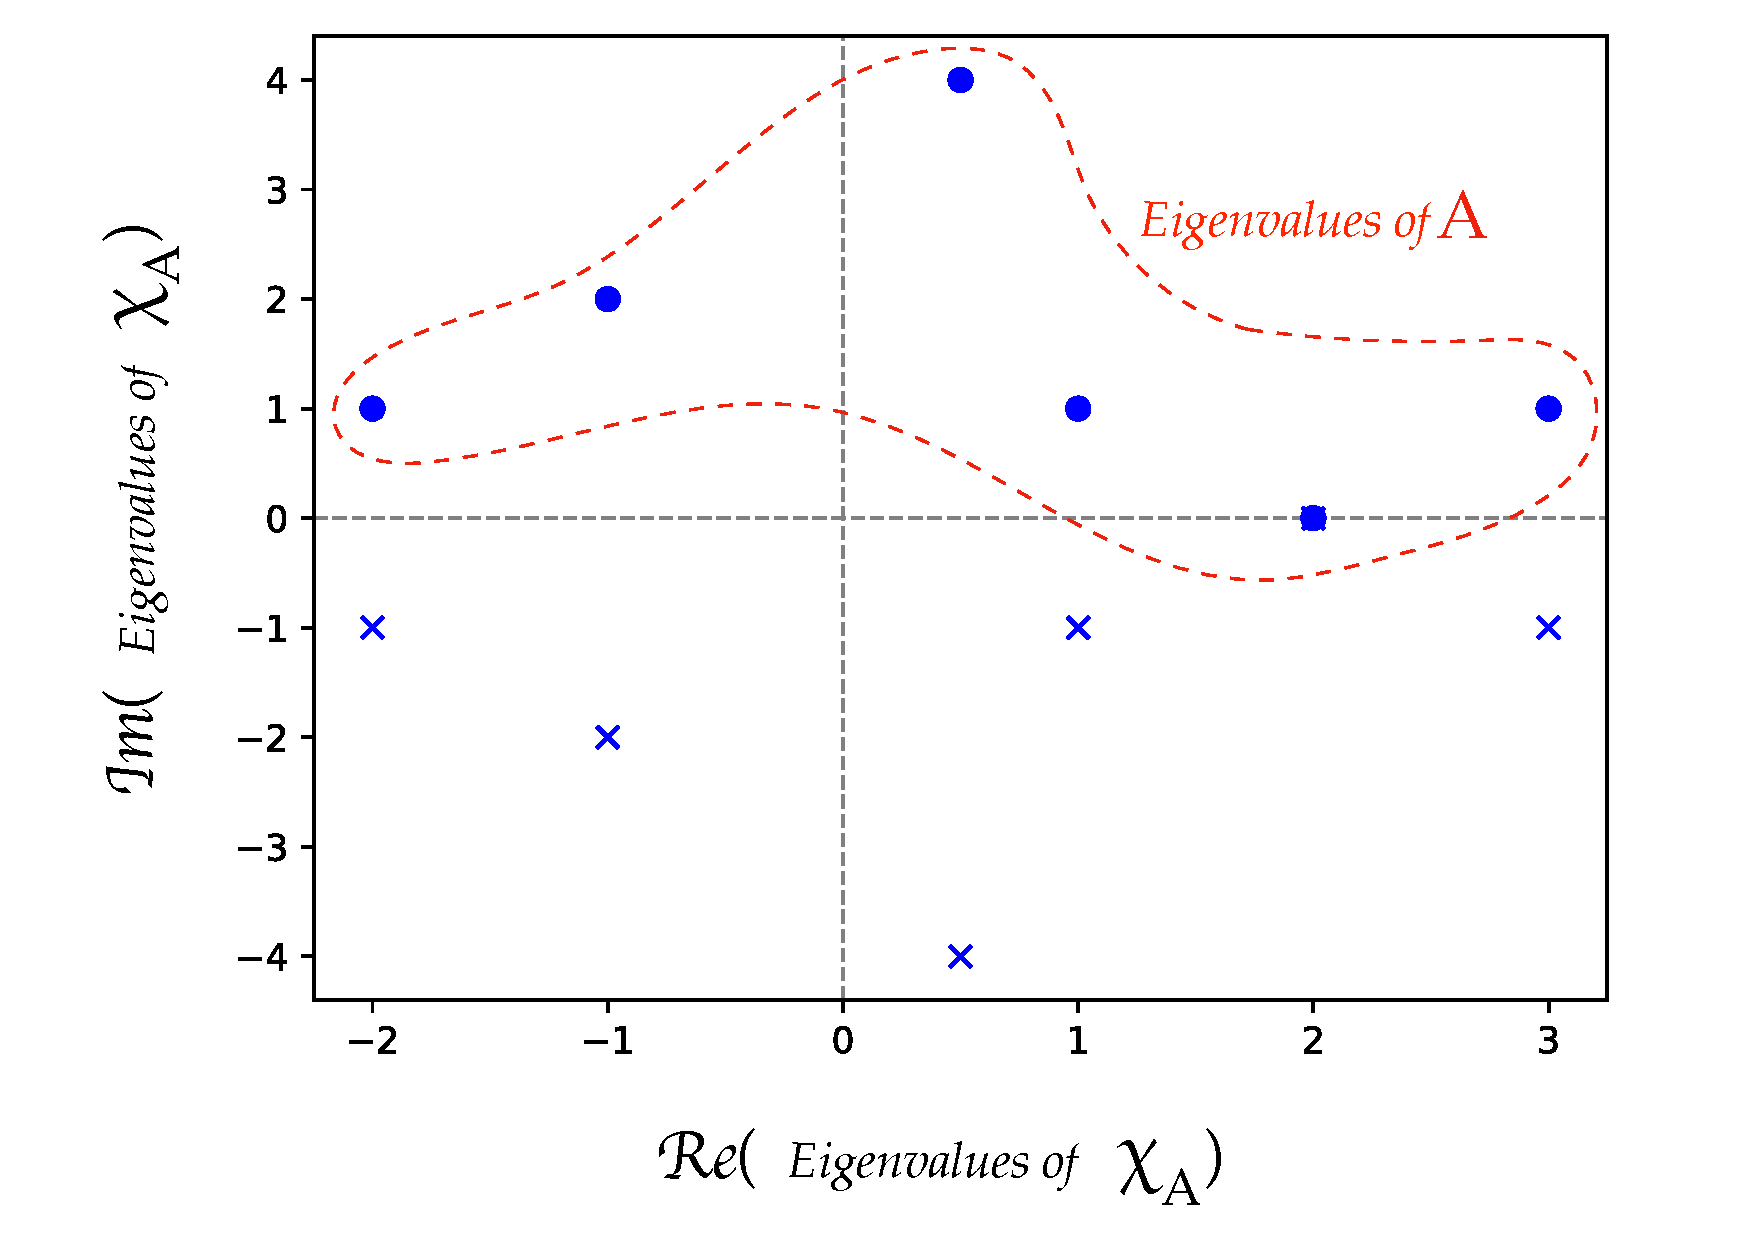
\includegraphics[width=0.7\linewidth]{Figures/complex_adjoint_eigvals_EN.pdf}
    \caption{\emph{Standard eigenvalues} of a quaternion matrix $ \mathbf{A} $, indicated as a subset of the eigenvalues of the complex adjoint matrix.}
\end{figure}


\begin{theorem}[\cite{zhang1997quaternions}]
    \label{th:02}
    Every matrix $ A \in \mathbb{H}^{n \times n} $ has exactly $ n $ right eigenvalues which are complex numbers with nonnegative imaginary parts. These are called the \textbf{standard eigenvalues} of $ \mathbf{A} $ and are a subset of the $ 2n $ eigenvalues of $ \rchi_A $.
\end{theorem}

\begin{proof}
    As demonstrated in the Appendix \ref{ch:AppendixA}, starting from the quaternion eigenvalue equation
    \begin{equation}
        \mathbf{A} \mathbf{v} = \mathbf{v} \lambda,
    \end{equation}
    in which one can assume without loss of generality that $ \lambda \in \mathbb{C} $, it is always possible to arrive at the \emph{equivalent} equation
    \begin{equation}
        \label{eq:eigvalueequation}
        \begin{pmatrix}
            \mathbf{A}_1              & \mathbf{A}_2            \\
            - \overline{\mathbf{A}}_2 & \overline{\mathbf{A}}_1
        \end{pmatrix}
        \begin{pmatrix}
            \mathbf{v}_1 \\
            - \overline{\mathbf{v}}_2
        \end{pmatrix} =
        \begin{pmatrix}
            \mathbf{v}_1 \\
            - \overline{\mathbf{v}}_2
        \end{pmatrix}
        \lambda,
    \end{equation}
    which involves solely complex-valued matrices and vectors, namely: the components of the symplectic decomposition of $ \mathbf{A} $ and $ \mathbf{v} $. The equivalence between both equations implies that $\mathbf{A}$ and its complex adjoint
    \begin{equation}
        \rchi_A =
        \begin{pmatrix}
            \mathbf{A}_1              & \mathbf{A}_2            \\
            - \overline{\mathbf{A}}_2 & \overline{\mathbf{A}}_1
        \end{pmatrix}
    \end{equation}
    \textit{share all their complex-valued eigenvalues} (notice that $\lambda$ remains unchanged as we move from one equation to its equivalent). As it appears, the eigendecomposition of the complex adjoint seems a promising method for finding some eigenvalues of the quaternion matrix.

    Is there, however, any possibility of leaving some eigenvalues behind? In other words, is it possible to exist some eigenvalue of $\mathbf{A}$ which does not belong to an eigenclass determined by a complex eigenvalue of $\rchi_A$? No, it is not, because it is always possible to align a quaternion's vector part with the $\qi$ axis through a single rotation (see Section \ref{subsec:rotacionando}). In other words,
    %all quaternions are similar to a specific complex number and, therefore,
    all (quaternion-valued) eigenvalues of $\mathbf{A}$ are similar to a complex number which, as discussed, must also be an eigenvalue of $\rchi_A$.

    Since $\rchi_A$ is a $ 2n \times 2n $-complex matrix, it has $ 2n $ complex-valued eigenvalues (possibly repeated). The reason why $\rchi_A$ share $2n$ eigenvalues with $\mathbf{A}$, even though $\mathbf{A}$ is an $ n \times n $ matrix is, once more, due to the existance of eigenclasses.

    According to \cite[Theorem 5]{lee1948eigenvalues}, the complex adjoint eigenvalues appear as $ n $ conjugate pairs (possibly some pairs are real-valued, so they are actually identical). Let us say that $2m$ of those eigenvalues are real, leaving $2(n-m)$ complex eigenvalues. Let $ q \in \mathbb{C}_{\qi}$ belong to the latter group. It can be shown imediately that $ q \sim \overline{q} $, since $ \overline{q} $ is obtained through a 180$ ^\circ $ rotation of the vector part of $ q $ around the $ \qj $ axis. This similarity transformation was already shown in (\ref{eq:commutej}), written as $\qj x = \overline{x} \qj$, or equivalently $\qj x (-\qj)= \overline{x}$. In the format of (\ref{eq:rotacao}), $ q \mapsto v q v^{-1} = \overline{q}$ with $ v = e^{\qj \frac{\pi}{2}} = \qj $.

    % (and so $ v^{-1} = e^{- \qj \frac{\pi}{2}} = -\qj $) to perform the simlarity transformation $ q \mapsto v q v^{-1} $,
    % \begin{equation}
    % \begin{aligned}
    % v q v^{-1} &= \qj (q_r + q_i \qi) (-\qj) = q_r - q_i \qj \qi \qj\\
    % &= q_r + q_i \qi \qj \qj = q_r - q_i \qi = \overline{q}.
    % \end{aligned}
    % \end{equation}
    Since two conjugate eigenvalues of $ \rchi_A $ are always similar, they belong to the same eigenclass and are therefore associated with the same set of linearly dependent eigenvectors. For that reason, by convention one can take the eigenvalues of $ \rchi_A $ and define the standard eigenvalues of $\mathbf{A}$ as being those complex-valued eigenvalues with positive imaginary part and half those real-valued ones.
\end{proof}

The following theorem is another fundamental result relating the eigenstructure of a quaternions matrix and that of its complex adjoint.

\begin{theorem}[Theorem 7.4 in \cite{zhang1997quaternions}]
    \label{th:diagonal}
    Given the matrices $ \mathbf{A}, \mathbf{B} \in \mathbb{H}^{n \times n} $, then $ \mathbf{A} $ is similar to $ \mathbf{B} $ if and only if $ X\rchi_A $ is similar to $ \rchi_B $.
\end{theorem}

\begin{corollary}
    \label{cor:diagonalizable}
    A matrix $  \mathbf{A} \in \mathbb{H}^{n \times n} $ is diagonalizable if and only if $ \rchi_A $ is diagonalizable.
\end{corollary}
\begin{proof}
    If $ \mathbf{A} \in \mathbb{H}^{n \times n} $ is diagonalizable, then it is similar to a diagonal matrix $ \Lambda \in \mathbb{C}^{n \times n}_{\qi} $ containing its standard eigenvalues in the main diagonal. From Theorem \ref{th:diagonal}, it follows that $ \rchi_A $ is similar to
    \begin{equation}
        \label{eq:Xlambda}
        \rchi_{\Lambda} =
        \begin{pmatrix}
            \Lambda    & \mathbf{0}         \\
            \mathbf{0} & \overline{\Lambda}
        \end{pmatrix},
    \end{equation}
    which is also a diagonal matrix. Therefore, $ \rchi_A $ is diagonalizable.

    On the other hand, if $ \rchi_A $ is diagonalizable, then it is similar to a diagonal matrix containing its $ 2n $ eigenvalues, which appear in $ n $ conjugate complex pairs. Therefore, its eigenvalues matrix may be written as (\ref{eq:Xlambda}), what implies, from Theorem \ref{th:diagonal}, that $ \mathbf{A} $ is similar to $ \Lambda $.
\end{proof}

\section{The quaternion Fourier transform}
\label{sec:QFT}
The field of quaternion signal processing has leveraged many tools to transform signals with quaternion-valued samples, from the fundamental redefinition of the gradient operador \cite{jiang2014general} up to algorithms for adaptive filtering \cite{jiang2013frequency}. This section focuses on the quaternion Fourier transform (QFT), as it is the basis for spectral analysis of quaternion signals.

Quaternion Fourier transforms have received quite a few definitions. Some are one-dimensional \cite{flamant2017spectral}, while others are intrinsically two-dimensional \cite{guanlei2008fractional}; the latter group can yet be divided into those having kernels oriented towards generic unit pure quaternions, and those using canonic imaginary units, such as $ \qi $ and $ \qj $. The 2D-transformed signals may be placed \textit{between} the two kernels or beside them. In fact, Ell \cite[sec. 3.2]{ell2014quaternion} lists 8 possibilities for the 2D-QFTs. The two dimensional case will not be covered for now, since the discussion on the 1D case already serves the purpose of introducing the main ideas and properties of this family of transforms.

Let $f$ be a quaternion-valued function $f: \mathbb{R} \rightarrow \mathbb{H}$ and $\qmu \in \qV(\mathbb{H})$, $\qmu^2 = -1$. The \textit{left} 1D QFT can be defined as the family of integral transforms
\begin{equation}
    \mathcal{F}^L_{\mp \qmu}[f](\omega) =
    F^L_{\mp \qmu}(\omega) \overset{def}{=}
    \kappa_{-} \int_{-\infty}^{\infty} e^{\mp \qmu \omega t} f(t) \mathrm{d}t.
    \tag{left 1D QFT}
\end{equation}

It can be proven that the inverse transform exists and is given by
\begin{equation}
    \mathcal{F}^{-L}_{\pm \qmu}[F^L](t) =
    f(t) =
    \kappa_{+} \int_{-\infty}^{\infty} e^{\pm \qmu \omega t} F^L(\omega) \mathrm{d}\omega.
    \tag{inverse left 1D QFT}
\end{equation}

In the expressions above, the unit pure quaternion $\qmu$ is called the \emph{eigenaxis} of the transform kernel, we could say it is the reference imaginary unit. The sign in the exponential is arbitrary, as long as the direct and inverse transforms use different signs. The real constants $\kappa_{-}$ and $\kappa_{+}$ satisfy
\begin{equation}
    \kappa_{+} \kappa_{-} = \frac{1}{2\pi},
\end{equation}
\noindent and when $\kappa_{-} = \kappa_{+}$, the transform is said to be unitary.

The right QFT may be defined likewise, by simply switching the relative positions of the kernel and the operand $f(t)$. The reader may notice that, when the eigenaxis is $\qi$, the QFT coincides with the usual continuous-time Fourier transform.

In this work, however, the most relevant version of the QFT is that in which both the original signal and its transformed representation are defined over discrete domains: the 1D quaternion discrete Fourier Transform (QDFT) with axis $ \qmu $, as defined in \cite[sec. 3.3.1]{ell2014quaternion}. If $ \qmu $ is a unit pure quaternion, the $ m $-th component of the transformed vector in the left unitary QDFT with axis $ \qmu $ is
\begin{equation}
    \label{eq:QDFT_fwd}
    \widehat{v}_m = \text{QDFT}\{ \mathbf{v} \}_m \overset{\Delta}{=} \frac{1}{\sqrt{N}} \sum_{n=0}^{N-1}  \exp \left( -\qmu \frac{2\pi}{N} nm \right) v_n \in \mathbb{C}_{\qmu},
\end{equation}
with inverse transform given by
\begin{equation}
    \label{eq:QDFT_inv}
    v_n = \text{QDFT}^{-1}\{ \widehat{\mathbf{v}} \}_n = \frac{1}{\sqrt{N}}\sum_{m=0}^{N-1}  \exp \left( \qmu \frac{2\pi}{N} nm \right) \widehat{v}_m.
\end{equation}

The transform analysis and synthesis equations may also be written in matrix form:
\begin{equation}
    \label{eq:QDFT}
    \widehat{\mathbf{v}} = \text{QDFT}\{ \mathbf{v} \} = \mathbf{F} \mathbf{v},
\end{equation}
\begin{equation}
    \label{eq:QDFT_mtx_inv}
    \mathbf{v} = \text{QDFT}^{-1}\{ \widehat{\mathbf{v}} \} = \mathbf{F}^{-1} \widehat{\mathbf{v}},
\end{equation}
in which $ \mathbf{F} $ is the unitary transform matrix,
%--multiplicando sempre \`a esquerda--,
with entries $ \{\mathbf{F}\}_{n,m} = \sqrt{N}^{-1} \exp \left( -\qmu \frac{2\pi}{N} nm \right)$. Since  $ \exp \left( -\qmu \frac{2\pi}{N} \right) $ is a $ N $-th root of unity, just like $ \exp \left( -\qi \frac{2\pi}{N} \right) $, it follows that $ \mathbf{F} $ shares many properties with the usual discrete Fourier transform (DFT) matrix, among which the invertibility, validating the existence of (\ref{eq:QDFT_inv}) and (\ref{eq:QDFT_mtx_inv}).

As it was done in previous pages, the symplectic decomposition may be applied to each entry of a quaternion matrix, generating complex-valued \emph{simplex} and \emph{perplex} matrices\footnote{Please note that, in what follows, the usual subscripts $1$ and $2$ for denoting the simplex and perplex parts were replaced by the superscripts $^{(s)}$ and $^{(p)}$, as in $q = q^{(s)} + q^{(p)} \qj$, to avoid confusion with the summation indices.}. Using this reasoning, Ell e Sangwine \cite{ell2014quaternion} demonstrated that the QDFT of a signal $ \mathbf{x} = [x_0, x_1, \dots, x_{N-1}] \in \mathbb{H}^N $ could be easily computed using two (complex) DFT, by decomposing each signal sample along the QDFT eigenaxis:
%. Relembrando a eq. (\ref{eq:QDFT_fwd}),
\begin{equation}
    \begin{aligned}
        %\label{eq:QDFT_fwd}
        \text{QDFT}\{ \mathbf{x} \}_m & = \frac{1}{\sqrt{N}} \sum_{n=0}^{N-1} \exp \left( -\qmu \frac{2\pi}{N} nm \right) x_n                         \\
                                      & = \frac{1}{\sqrt{N}} \sum_{n=0}^{N-1} \exp \left( -\qmu \frac{2\pi}{N} nm \right) (x_n^{(s)} + x_n^{(p)}\qnu) \\
                                      & = \text{DFT}_{\qmu}\{ \mathbf{x}^{(s)} \}_m +
        \text{DFT}_{\qmu}\{ \mathbf{x}^{(p)} \}_m \qnu,
    \end{aligned}
\end{equation}
in which $ \text{DFT}_{\qmu} $ indicates the DFT computed with ``complex numbers'' having $ \qmu $ as imaginary unit.
Although that statement is technicaly incorrect (complex numbers strictly belong to $\mathbb{C}_{\qi}$), from a computational point of view, the $ \text{DFT}_{\qmu} $ can be calculated using the very same algorithms as the usual DFT (since the imaginary unit \textit{per se} is disregarded in the low-level calculations).

This brief presentation of the QDFT illustrates that
\begin{itemize}[noitemsep]
    \item although the frequency components are quaternion signals, their frequencies are real-valued (see the argument in the transform kernel),
    \item the eigenstructure of the QDFT likens heavily that of the usual DFT, to the point of allowing the reuse of common DFT algorithms. This resemblance will be exploited when investigating the fractionalization of the QDFT, in Chapter \ref{ch:FrQDFT}.
\end{itemize}

For a thorough introduction on quaternions and their application to signal processing, the reader may refer to \cite{grigoryan2018quaternion,zhang1997quaternions,ell2014quaternion,flamant2017time, jiang2014general}.

\section{Summary}

This chapter discussed the main topics concerning the quaternion algebra and its Fourier transform. Although they have not been addressed with the depth and details a more curious reader would wish, the discussion was hopefully enough to present a coherent overview of
\begin{itemize}[noitemsep]
    \item how the quaternions extend the complex numbers, by carrying not 2 but 4 real-valued components splitted into a scalar and a vector part,
    \item how the quaternion multiplication rules effect the quaternion similarity classes, with their rotation property,
    \item how the symplectic decomposition and the complex adjoint matrices are core concepts in the eigendecomposition of a quaternion matrix, and
    \item how to compute the left 1D discrete quaternion Fourier transform by using usual DFT calculations.
\end{itemize}